%%%%%%%%%%%%%%%%%%%%%%%%%%%%%%%%%%%%%%%%%%%%%%%%%%%%%%%%%%%%%%%%%%%%%%%%%%%%%%%%%%%%%%%%%%%%
%%
%% Chapter 5 : Current progress
%%
%%      * Should describe the current state we are in the implementations, research, etc.
%%
%%%%%%%%%%%%%%%%%%%%%%%%%%%%%%%%%%%%%%%%%%%%%%%%%%%%%%%%%%%%%%%%%%%%%%%%%%%%%%%%%%%%%%%%%%%%

\chapter{Current progress}
\label{ch:current_progress}

%%%%%%%%%%%%%%%%%%%%%%%%%%%%%%%
%   Figures for chapter 5
%%%%%%%%%%%%%%%%%%%%%%%%%%%%%%%

\newcommand{\figProgressAgents}{
    \begin{figure}
        \centering
        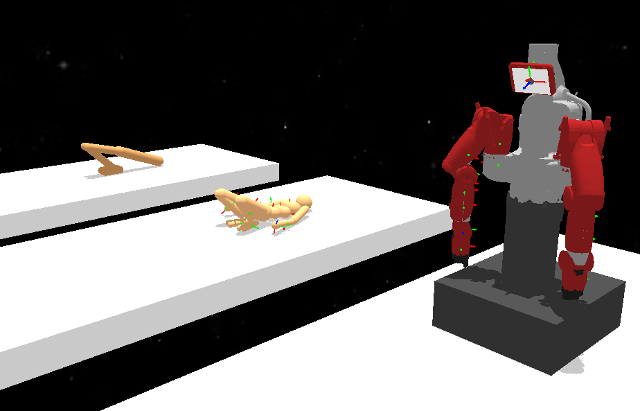
\includegraphics[width=0.9\textwidth]{./chapters/chapter_5/imgs/img_tysocmjc_agents.png}
        \caption{Current agent support. Currently the framework support mjcf
                 formats (from the mujoco engine)}
        \label{fig:ch5_progress_agents}
    \end{figure}
}

\newcommand{\figProgressSensors}{
    \begin{figure}
        \centering
        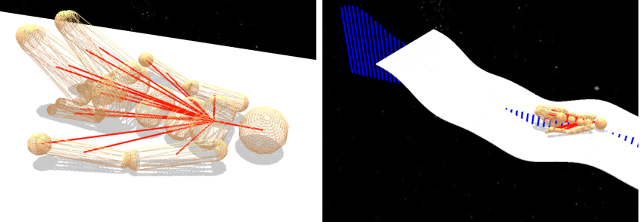
\includegraphics[width=0.9\textwidth]{./chapters/chapter_5/imgs/img_tysocmjc_sensors.png}
        \caption{Current sensor support. Currently the framework supports: 
                            a) intrinsic measurements (joint angles and velocities, body velocities and acceelrations, and relative positions).
                            b) extrinsic measurements (height fields taken from the terrain)}
        \label{fig:ch5_progress_sensors}
    \end{figure}
}

\newcommand{\figProgressTerrains}{
    \begin{figure}
        \centering
        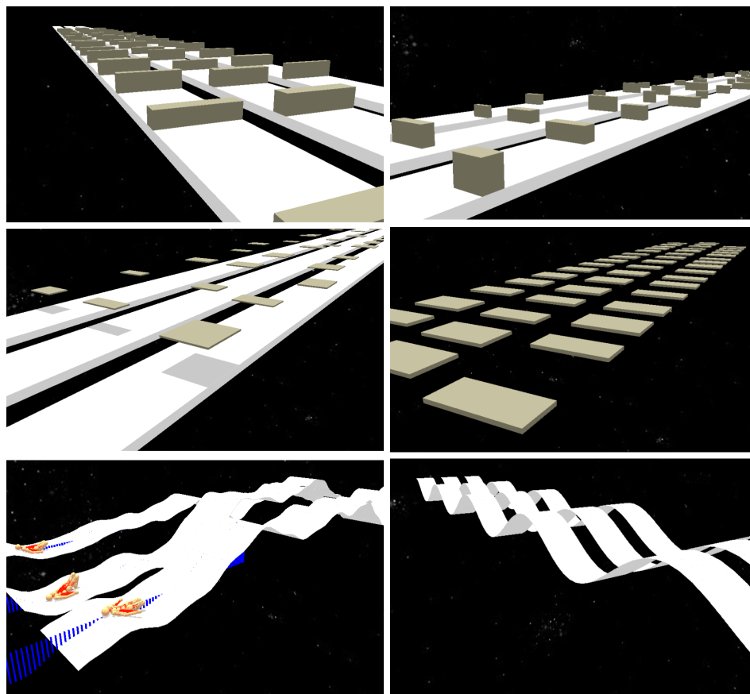
\includegraphics[width=0.9\textwidth]{./chapters/chapter_5/imgs/img_tysocmjc_terrains.png}
        \caption{Current terrain support. Currently the framework supports the
                 environments from \citeauthor{DeepmindEmergenceLocomotion}}
        \label{fig:ch5_progress_terrain}
    \end{figure}
}

\newcommand{\tableAgentFormatsSupport}{
    \begin{table}[]
        \centering
        \begin{tabular}{c|c|c|c|}
        \cline{2-4}
                                        & \cellcolor[HTML]{C0C0C0}{\color[HTML]{333333} mjcf} & \cellcolor[HTML]{C0C0C0}{\color[HTML]{333333} urdf} & \cellcolor[HTML]{C0C0C0}{\color[HTML]{333333} rlsim} \\ \hline
        \multicolumn{1}{|c|}{Completed} & x                                                   & x                                                   &                                                      \\ \hline
        \multicolumn{1}{|c|}{Tested}    & x                                                   &                                                     &                                                      \\ \hline
        \end{tabular}
        \caption{Current agent formats supported in the framework}
        \label{tab:ch5_table_supported_agent_formats}
    \end{table}
}

\newcommand{\tableBackendsSupport}{
    \begin{table}[]
        \centering
        \begin{tabular}{c|c|c|}
        \cline{2-3}
                                        & \cellcolor[HTML]{C0C0C0}{\color[HTML]{333333} MuJoCo} & \cellcolor[HTML]{C0C0C0}{\color[HTML]{333333} Bullet} \\ \hline
        \multicolumn{1}{|c|}{Completed} & x                                                     &                                                       \\ \hline
        \multicolumn{1}{|c|}{Tested}    & x                                                     &                                                       \\ \hline
        \end{tabular}
        \caption{Current backends supported in the framework}
        \label{tab:ch5_table_supported_backends}
    \end{table}
}

In this chapter we discuss the current progress of the proposed framework. 
The implementation is still not in version 0.1, which should be the first 
fully functional version to be released according to the features proposed 
in the previous chapter. Nevertheless, the core functionality, which is related
to the abstract representations (section ~\ref{subsec:ch4_core_functionality}),
is working and almost completed. There is also a working implementation for
MuJoCo, one of the two backends that we will support.

All the implementations are available in github, in the following repositories:

\begin{itemize}
    \item \textbf{Core functionality}, which is the repository that serves as the
          core dependency for the framework. It can be found \href{https://github.com/wpumacay/tysocCore}{here}.
    \item \textbf{MuJoCo implementation}, which is the repository with the
          adapter code for MuJoCo as the specific backend. It can be found
          \href{https://github.com/wpumacay/tysocMjc}{here}.
\end{itemize}

\section{Core functionality}

As previously mentioned we already have a working implementation of the core
functionality supporting part of the proposed agent formats, the appropriate
abstractions for the terrain and sensors, and this is decoupled of the specific
backend we used for testing. The key points currently available are:

\begin{itemize}
    \item \textbf{Agent core functionality}: We implemented the core kinematic 
            tree (see Figure ~\ref{fig:ch4_core_agent_functionality}), and currently
            have support for the \textbf{mjcf} and \textbf{urdf} agent formats.
            We have also support for three agents from the proposed agents list:
            walker and humanoid from Controlsuite, and laikago from PyBullet. These
            are shown in the Figure below.

            \figSupportedAgents

\end{itemize}

@TODO: talk about the impl. of the core kintree and currently supported formats
@TODO: make a table to list done and todos in this feature

@TODO: talk about the visualizer, and the two implemented options.
@TODO: make a table to list done and todos in this feature

@TODO: talk about the backends supported so far
@TODO: make a table to list done and todos in this feature

\section{Features}

\subsection*{Agents support}

The implementation of the agent's core functionality has been completed to a 80\%,
remaining only an additional implementation of the agents format provided by \cite{TerrainRLSim}.
This implementation includes the agent's kinematic tree implementation and the integration 
with the MuJoCo physics engine via an adapter written for this specific engine.

The core implementation remains agnostic of the specific engine, which allows us
to make support quickly for the remaining proposed physics engines via adapter code
written once for each platform. The current supported agents are shown in Figure ~\ref{fig:ch5_progress_agents},
which basically shows the support for agents made for MuJoCo via its XML representation format.

The current implementation can be already used for experiments from C/C++. The exposed
functionality includes the supported functionality exposed by most benchmarks, which
give access to the actions via torques. The remaining part of the implementation of the core
agent functionality should give more support for different types of actuation models, like in \cite{ActuationChoice}.

\figProgressAgents

\subsection*{Sensors support}

The implementation of the sensors' core functionality is completed to a 70\%,
remaining some sensors for more complicated tasks: visual inputs from a fixed camera,
and heightmap measurements from more complicated terrains. The current supported sensor
features shown in Figure ~\ref{fig:ch5_progress_sensors}, and consist of:

\begin{itemize}
    \item Intrinsic sensor measurements, like joints angles and velocities, bodies velocities
          and accelerations, and bodies relative positions (to the root body).
    \item Extrinsic sensor measurements, which consist on heightfield data from the terrain ahead,
          taken with respect to the root body.
\end{itemize}

\figProgressSensors

\subsection*{Terrain support}

The current implementation of the core terrain functionality supports procedurally generated
terrain, similar to \cite{DeepmindEmergenceLocomotion}. The core functionality handles 
the creation of primitives from terrain generators, and then this is stored as 
requests for creation in the specific adapters for specific engines. The current 
supported engine is MuJoCo, and we plan in adding full support for more complex 
terrains (and an API to use it), and full support for the remaining proposed physics 
engines. Some screenshots of the current terrain implementations are shown
in Figure ~\ref{fig:ch5_progress_terrain}.

\figProgressTerrains

\todo{deberías cerrar el capítulo con una discus ión breve de lo que se hizo}

\tableAgentFormatsSupport
\tableBackendsSupport